%===============================================================================
%  Cyclade 3 : environnement de développement
%===============================================================================
\documentclass[10pt]{smile}
\usepackage[utf8]{inputenc}
\usepackage[OT1]{fontenc}
\usepackage[french]{babel} 
\usepackage{codes}
\usepackage{multicol}




%-------------------------------------------------------------------------------
% VERSIONS
%-------------------------------------------------------------------------------
\title{YouTestIt Développement}
\setversion{%
\major[v1]{30/10/2011}{Patrick Guillerm}{Initialisation du document}
}

\newcommand{\youTestIt}{\emph{YouTestIt}}

\newcommand{\positif}{ \includegraphics[width={0.015}\textwidth]{{positif}}}
\newcommand{\negatif}{\includegraphics[width={0.015}\textwidth]{{negatif}}}

%===============================================================================
% document :
%===============================================================================
\begin{document}
\makefront

%-------//Chapter : introduction //---------------------------------------------
%===============================================================================
% Smile Selenium introduction
%===============================================================================
\newpage{}
\chapter{Introduction}

\section{Le but du projet}

L'intégration continue est un point très important dans le développement d'application pour limité
les bugs. On améliore ainsi la qualité des projets et facilite grandement les livraisons. 

\youTestIt{} fait partie des outils d'intégration continue, en permettant de tester les actions que les
utilisateurs feront sur l'application. Il permet de gérer les campagnes de tests ainsi que de l'automatiser.
L'automatisation des tests se fait via Selenium \footnote{Selenium est un outils permettant l'écriture et
l’exécution de tests sur un navigateur web}. 


\youTestIt{}  est une application WEB, cela permettant un déploient simplifier et un travail en équipe bien
plus simple. La création et la maintenance des tests Selenium peut rapidement devenir très complexe,
il est nécessaire d'avoir un outils facilitant ce processus.

\youTestIt{} a deux objectifs principaux :
\begin{itemize}
	\item Facilité la création et maintenance des tests Selenium  en apportant une approche fonctionnelle.
	\item D'aider à mesurer la qualité d'un projet.
\end{itemize}



Les clients sont rarement des développeurs expérimenter, ils ont besoin d'un outils
qui leurs permettent de concevoir des tests d'un point de vue fonctionnel, et ceux
sans que les contraintes techniques ne freinent leurs taches. 

Cette outils permet également d'améliorer la relation cliente, en les faisant participer
à la vie du projet (descriptions et conceptions de tests Selenium), ou en leurs donnant 
une meilleure vision de l'évolution de la qualité de leurs projets. 

Un point qui est souvent complexe et couteux en temps est le fait de tester un projet 
sur les différents navigateurs cibles.  Le fait d'avoir un outils qui est capable d'exécuter
des tests sur différents plateformes avec une configuration simple est un réel avantage.
Selenium permet de lancer des tests sur différents systèmes d'exploitations et navigateurs, 
cependant la configuration n'est pas simple pour des personnes n'ayant pas des notions 
d'administration système. 

La parallélisation des calculs est également un point important.  Un test Selenium prend du 
temps à s'exécuter. Imaginons que l'on ait  beaucoup de tests avec différents navigateurs, le
temps nécessaire sera conséquent. En distribuant les calculs sur différents machines, le temps
nécessaire pour effectuer l'ensemble de ces tests sera considérablement réduit. 

\begin{description}
	\item \positif{}
	  Approche fonctionnelle des tests Selenium, ne nécessite pas de connaissant approfondie en développement.
	\item \positif{}  Gestion des tests Selenium simplifié.
	\item \positif{}  Tests sur différents environnements plus simple à configurer.
	\item \positif{}  Meilleur vision de l'évolution de la qualité d'un projet (statistiques plus complètes).
	\item \positif{}  Évite les régressions, extrêmement important dans le cadres de TMA.
	\item \positif{}  Améliore la relation clients (participation à la création des tests et ou meilleur vision de la qualité du projet)
\end{description}


%-------//Chapter : technicalChoice //-----------------------------------------
%===============================================================================
% Technical Choice
%===============================================================================
\newpage{}
\chapter{les choix techniques}


%*******************************************************************************
\section{Les frameworks :}
%*******************************************************************************

L'application contient beaucoup d'écrans assez complexe, avec formulaires,
des diagrammes, composants divers. Pour ce type d'application il est nécessaire
d'avoir un framework qui aide le développement, et permet une grande productivité.

Le nombre d'utilisateur simultané est assez limité , il n'y a donc pas de raison
d'utiliser un framework Statless\footnote{Framework donc les pages n'ont pas d’état}.

La framework MVC ne permettent pas une intégration simple et performante de composants
graphique complexes (diagramme par exemple). Le formulaires et l'ajax reste le gros point
faible de ces frameworks.

Un framework orienté composants correspondrait d'avantage aux divers problèmes techniques. 
Ce type de framework facilite énormément la création de formulaires. Ils ont souvent un 
framework Ajax interne, évitant ainsi l'écriture de code javascript. Ce point est très important
pour la maintenance de l'application. Mais le point le plus important de ces frameworks est
la possibilité de découper une application en petites briques réutilisables. Leurs bibliothèques
de composants facilite la création d'interfaces riches.


Il existe différents frameworks composants :
\begin{itemize}
	\item \bold{Google GWT :}
		Très en vogue, mais comporte un problème majeur : sa productivité. GWT permet d'
		avoir des pages compatible avec la plus part des navigateurs. Pour cela, GWT génère
		la page entièrement en javascript. Ce  point pose différent  problèmes, comme le fait
		qu'il est difficile d'appliquer une charte graphique à GWT. Il nécessite également beaucoup
		de fichiers pour réaliser un composant.
		\\
		
	\item \bold{Tapestry 5 :}
		C'est un très bon framework, axé sur de la convention, limitant la configuration XML.
		Il est léger et performant, mais la prise en main est un peu complexe, et peut de développeurs
		connaissent ce framework.
		\\
		
	\item \bold{Wicket :}
		Wicket a un très bon système de templating, qui permet d'intégrer rapidement des pages
		html. Cependant le coté java est rapidement très verbeux. Pour des applications complexe
		cela peut amener des risques sur la maintenabilité. 
		\\

	\item \bold{Seam 3 / JSF2 :}
		Seam et JSF sont devenu les standard de la norme JEE 6. Ce framework facilite énormément
		l'intégration de formulaires complexes, et possède une collection de composants conséquent. 
		C'est également l'une des technologie les plus simple pour la création de composant (via les
		composants composites). Les liaisons entre le frontal, le coeur du framework et la persistance
		y sont très bien gérées. Cependant beaucoup de développeurs ont des aprioris sur cette technologie.
		En effet JSF 1.1 et les EJB 2 ont laissé beaucoup de mauvais souvenir. Ce framework est également
		conçue pour un environnement JEE. Mal-grès les idées reçu Seam et JSF sont des frameworks
		extrêmement productif, simple et performant. 

\end{itemize}


\newpage{}
Le choix se porte donc sur :
\begin{itemize}
	\item \bold{Seam 3 - JEE 6 :}
		pour sa capacité modulaire, sa faible configuration XML, la capacité de gestion des divers 
		couches applicatives. De plus c'est un framework reposant sur les standards de la norme JEE.
		\\
		
	\item \bold{JPA 2 :}	
		Seam a été conçu pour fonctionner avec JPA\footnote{Java Persistence API}. JPA permet la persistance de données, et aide
		au mapping entre le modèle objet et le modèle relationnelle des bases de données. Sa configuration
		est essentiellement baser sur des annotations, limitant la configuration XML. Il est également
		possible de l'associer à Hibernate Search pour les recherches full text ainsi que la
		JSR-303\footnote{Validation par annotations} bean
		validator pour la validation des formulaires. JPA et JSF 2 sont totalement compatible avec 
		la validations par annotations (JSR-303).
		\\
		
	\item \bold{JAX-RS :} pour les services REST de l'application.
		\\
		
	\item \bold{JSF 2 :}
		Ce framework  permet un templating et un découpage par composants. Cette technologie est très 
		productive pour tout ce qui touche aux formulaires et permet un intégration élégante
		d'Ajax. Le projet Facelets y a été intégré nativement, ce qui permet la conception 
		de Layout, et d'héritage entre différent layouts. De plus cette technologie fait
		partie intégrante de la norme JEE 6.
		\\
			    			
	\item \bold{ Richfaces 4 / Primefaces 3 :}
		Ce tandem de bibliothèque de composants est conçu pour fonctionner ensemble. Primefaces
		apporte énormément de composants (diagramme, upload en html 5, etc...). Richfaces apporte
		toutes la parties abstraction Ajax, qui permet d'avoir des composants riches sans que l'on ait 
		besoin d'écrire de code javascript. La maintenance en est considérablement améliorée. 
		\\
				
	\item \bold{PostgreSQL :}	 C'est la base de données Open Source la plus performante.
		\\
			
	\item \bold{JBoss 7 :}
		JBoss ont fait énormément d'optimisation sur leur serveur d'application,  principalement
		sur l'utilisation multi-coeurs des processeurs. Il est également un serveur compatible avec la
		norme JEE 6, ainsi que l'implémentation de référence pour le class loader (JBoss Weld).
		\\

		
	\item \bold{HTML 5 :}
		Pour profiter au maximum des composants de primefaces, l'application se doit d'être en
		HTML 5, de plus il faut respecter un maximum l'ergonomie et l'accessibilité. 
		\\
						
	\item \bold{JBoss cache / Ehcache :}
		Seam permet une optimisation via l'utilisation du cache JBoss. Ce cache permet d'utiliser
		différente implémentation. Ehcache permet une grande finesse de configuration. Seam
		permet également d'utiliser Ehcache dans les templates JSF.
\end{itemize}



%+++++++++++++++++++++++++++++++++++++++++++++++++++++++++++++++++++++++++++++++
\section{Environnement systèmes :}
%+++++++++++++++++++++++++++++++++++++++++++++++++++++++++++++++++++++++++++++++

\subsection{Packaging}
L'environnement nécessaire au fonctionnement de l'application reste assez classique, 
elle nécessite un serveur d'application ou conteneur de servlets. Toute fois. Les applications
JEE 6 peuvent aussi bien être sous forme d'EAR\footnote{Enterprise Application ARchive}   ou de 
WAR\footnote{Web Application ARchive}.

Dans un premier temps \youTestIt{} sera sous forme de WAR, une version EAR sera conçu ultérieurement.


\subsection{Le serveur}
Le serveur de référence est JBoss 7 (7.0.2.Final ou supérieur en packaging \textbf{Everything}). 
Le serveur se doit de rester standard et avec un minium de configuration (configuration de la data
source reste nécessaire).



%-------//Chapter : technical environnement //----------------------------
%===============================================================================
% Technical Environnement
%===============================================================================
\newpage{}
\chapter{Environnement de développement}

%+++++++++++++++++++++++++++++++++++++++++++++++++++++++++++++++++++++++++++++++
\section{Eclipse - indigo}
%+++++++++++++++++++++++++++++++++++++++++++++++++++++++++++++++++++++++++++++++
Le développement de \youTestIt{} est réalisé sous eclipse avec différents plugins afin de standardiser 
le code. Il est préférable pour toutes contributions d'utiliser un environnement similaires.

La version utiliser doit être une version supérieur ou égale à \textbf{indigo}. 

Liste des plugins :
\begin{itemize}
	\item JBoss tools : qui permet l'intégration simple de jboss 7 ainsi que des outils pour Seam.
				Le plugin est présent sur le marcket place d'eclipse.
				
	\item Maven Integration for Eclipse : pour la gestion des dépendances.
					Le plugin est présent sur le marcket place d'eclipse.
					
	\item EGit : pour la gestion des sources sous GitHub
					Le plugin est présent sur le marcket place d'eclipse.
					
	\item PMD : pour la vérification du code
					Le plugin s'installe via l'adresse \textbf{http://pmd.sourceforge.net/eclipse } à rajouter dans 
					le menu software update d'eclipse.
					
	\item Check style : pour la vérification du code
					Le plugin est présent sur le marcket place d'eclipse.
					
	\item Grep Console : non obligatoire, mais facilite la lecture de la console
					Le plugin est présent sur le marcket place d'eclipse.
\end{itemize}

\paragraph{Formatage du code :}
Il est très important de configurer eclipse avec les différents fichiers de formatages
présent dans le projet. 

On retrouve cinq fichiers de configuration :
\begin{itemize}
	\item  \textbf{cleanups.xml :}  Se configure dans : ((\leftArrow{}))
				  preferences \rightArrow{} Java \rightArrow{}Code Style\rightArrow{}Clean up

	\item \textbf{codetemplates.xml :}  Se configure dans :
				 preferences \rightArrow{}Java \rightArrow{}Code Style\rightArrow{}Code template

	\item \textbf{formatter.xml :} Se configure dans :
				 preferences \rightArrow{} Java \rightArrow{}Code Style\rightArrow{}Formatter

	\item  \textbf{pmd.xml :} Pour tous les projets importés il faut aller dans leurs propriétés  
		(clique droit sur le projet\rightArrow{}Properties ).
		\begin{enumerate}
			\item aller dans le menu PMD
			\item cliquer sur "activer PMD"
			\item il faut en suite cliquer sur \emph{Utiliser l'ensemble des règles configuré dans un fichier projet}
			\item cliquer sur parcourir pour rechercher le fichier de configuration du projet.
			\item valider le formulaire.
		\end{enumerate}


	\item  \textbf{checkstyle.xml :}
		Pour le configurer il faut suivre les étapes suivantes :
		\begin{enumerate}
				\item aller dans les préférences d'eclipse
				\item aller dans menu Checkstyle
				\item cliquer sur new
				\item une nouvelle fenêtre s'ouvre, il faut choisir \textbf{External Configuration File}
				\item donner un nom à la configuration
				\item cliquer sur \textbf{Browse...} pour aller rechercher le fichier checkstyle.xml du projet \youTestIt{}.
				\item valider le formulaire.
				\item définisser la nouvelle configuration comme configuration par défaut (\textbf{Set as Default})
				\item A présent pour chaque projet importer il faut aller sans sa configuration 
							(clique droit sur le projet\rightArrow{}Properties )
				\item Dans le menu Checkstyle  il faut choisir la configuration  \youTestIt{} et valider le formulaire.
		\end{enumerate}
	

	\paragraph{}	
	
	\begin{attention}
		Toute contribution ne respectant pas les conventions de formatage ne sera pas prit en compte.
	\end{attention}
	
\end{itemize}
%+++++++++++++++++++++++++++++++++++++++++++++++++++++++++++++++++++++++++++++++
\section{GitHub}
%+++++++++++++++++++++++++++++++++++++++++++++++++++++++++++++++++++++++++++++++
L'ensemble du code source du projet se trouve sur GitHub. Pour pouvoir contribuer il est
nécessaire d’être inscrit sur le site.  Une fois inscrit il faut crée et uploader sa clé RSA, pour cela il faut suivre le tutoriel proposé 
par GitHub : \href{http://help.github.com/linux-set-up-git/ }{http://help.github.com/linux-set-up-git}. 

une fois le compte gitHub configuré, il suffit de faire une demande d'ajout par mail à l'adresse
\textbf{administrator@youtestit.org}, pour que l'on vous rajoute au projet.

\subsection{Configuration eclipse pour GitHub}
Une fois ajouter sur le projet  vous pouvez récupérer les sources et commencer à contribuer. 
Mais avant cela il faut encore configurer eclispe pour avoir un environnement de développement
fonctionnel. 

\begin{enumerate}
	\item créer un dossier dans votre home (par exemple : /home/yourLogin/git ). Ce dossier contiendra
	 l'ensemble des sources du projet.
	 
	\item Il faut ensuite cloner tous les projets dans ce dossier
	 \lstsetSh{}
	 \lstinputlisting{includes/src/gitClone.sh}
	 
	 \item Le plugin EGit fonctionne très mal avec la librairie SSH d'eclipse, il faut impérativement lui
	 ordonner de travailler avec la librairie système. Pour cela il faut  crée un script shell pour le lancement
	 d'éclispe qui va initialiser les bonnes variables d'environnement.
	 
	 \lstsetSh{}
	 \lstinputlisting{includes/src/eclipse.sh}
	On en profite également pour spécifier l'emplacement de maven et du JDK.
	\newpage

	 \item Une fois eclipse démarrer on va pouvoir récupérer nos dépôt git. Dans la perspective
	 Git repository exploring, on peut rajouter un dépôt en cliquant sur l'icone avec un + vert.
		\begin{figure}[!h]
     		\begin{center}
			      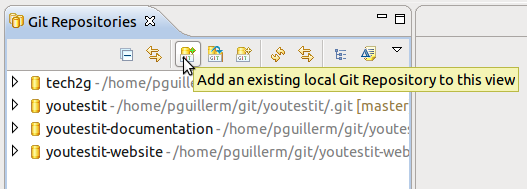
\includegraphics[width=0.5\textwidth]{gitAdd}
			      \caption{Ajout d'un dépôt Git}
			      \label{gitAdd}
		    \end{center}
		\end{figure}
		
	 \item Une nouvelle fenêtre s'ouvre dans la quel on va pouvoir aller chercher  l'emplacement du
	 dépôt Git locale. Le bouton "seach" permet au plugin d'aller récupérer le .git du dépôt. Il ne 
	 reste plus qu'à valider le formulaire.
		\begin{figure}[!h]
     		\begin{center}
			      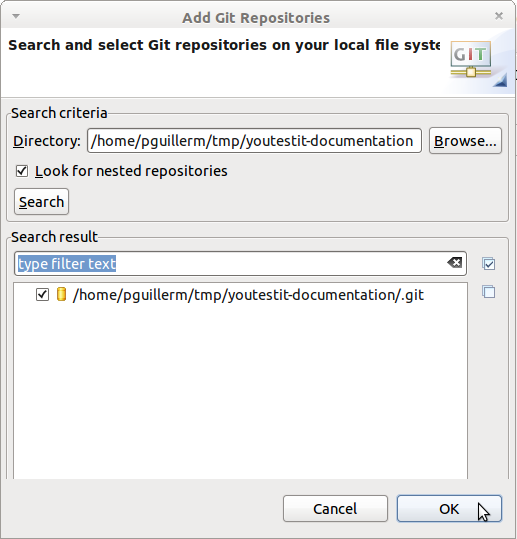
\includegraphics[width=0.5\textwidth]{gitRepo}
			      \caption{Récupération des dépôt Git}
			      \label{gitAddRepo}
		    \end{center}
		\end{figure}
		\newpage
	 
	 \item Git a besoin d'une connexion SSH avec une clé RSA pour fonctionner. Il faut
	 bien vérifier que la configuration eclipse pour SSH est correcte et qu'elle contient
	 bien la clé RSA.
		\begin{figure}[!h]
     		\begin{center}
			      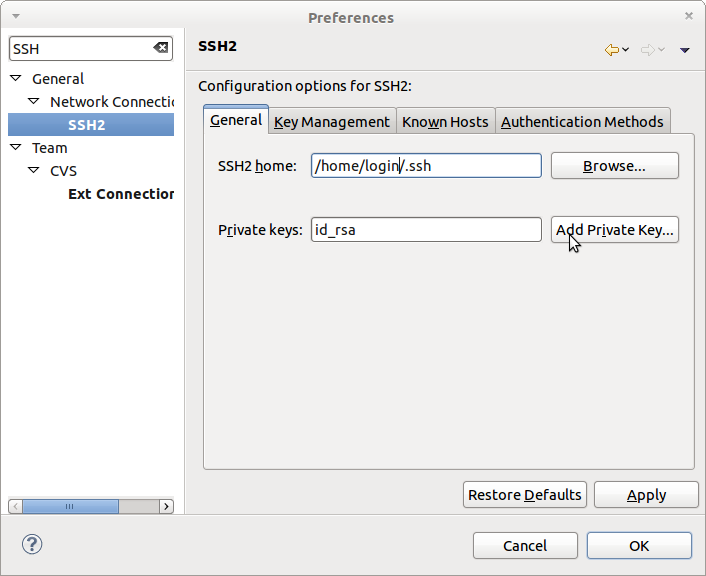
\includegraphics[width=0.5\textwidth]{sshParams}
			      \caption{Configuration SSH d'eclipse}
			      \label{eclipseSshConfig}
		    \end{center}
		\end{figure}		 
	 
	\item Une fois la configuration terminée, vous pouvez importer les projets en tant que "general project" .
	Pour cela il suffit de déplier le dépôt et de faire un clique droit sur le "Working directory" .
		\begin{figure}[!h]
     		\begin{center}
			      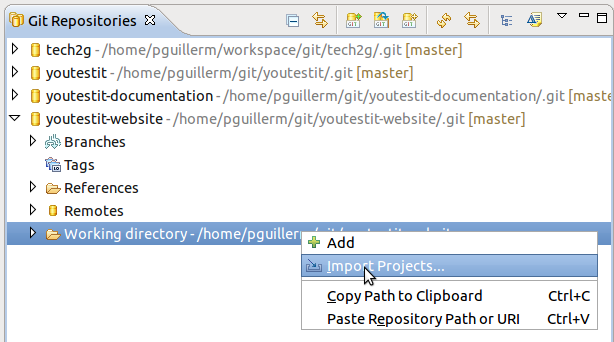
\includegraphics[width=0.5\textwidth]{importProject}
			      \caption{Importation d'un projet}
			      \label{gitProjectImport}
		    \end{center}
		\end{figure}	
		
	\item Votre environnement est prêt à faire de pull et push ;)   Pour plus  d'information je vous invite à lire la
	documentation du plugin Egit : \href{http://wiki.eclipse.org/EGit/User\_Guide}{http://wiki.eclipse.org/EGit/User\_Guide} . 
 
	 
\end{enumerate}

%+++++++++++++++++++++++++++++++++++++++++++++++++++++++++++++++++++++++++++++++
\section{youtestit-documentation}
%+++++++++++++++++++++++++++++++++++++++++++++++++++++++++++++++++++++++++++++++
Le projet \textbf{youtestit-documentation} est celui qui contient l'ensemble de la documentation
technique et fonctionnel. Les différents fichiers sont écris en LaTeX afin de permettre un meilleur
découpage et la possibilité d'exporter les documentations sur différents formats (PDF, html, text brut).


Les sources LaTeX sont re-compilées  quotidiennement  via la plateforme d'intégration continue

(\href{http://youtestit.org/jenkins/job/youtestit-documentation/}
		     {jenkins})

La conversion en HTML est fait via un fork du projet tex Konverter (
		\href{http://www.texconverter.org}{www.texconverter.org}). La base de ce projet est bien
conçu, est fonctionne plutôt bien. Cependant certaines fonctionnalité n'étaient pas implémentées,
comme la gestion des sources, ou des footnote, etc... Nous sommes en cours d'y remédier et
reverserons une fois le fork terminé. 

%+++++++++++++++++++++++++++++++++++++++++++++++++++++++++++++++++++++++++++++++
\section{youtestit-website}	
%+++++++++++++++++++++++++++++++++++++++++++++++++++++++++++++++++++++++++++++++
Le projet Youtestit-website est la partie web présent à l'url \href{http://www.youtestit.org}{www.youtestit.org}.
A l'heur actuelle le site est constitué de page web statiques, nous étudions la possibilité de les
remplacer par une solutions de CMS OpenSource (surement basé sur \href{http://www.onehippo.com/en/products/cms}{HippoCMS}). 



%+++++++++++++++++++++++++++++++++++++++++++++++++++++++++++++++++++++++++++++++
\section{youtestit}
%+++++++++++++++++++++++++++++++++++++++++++++++++++++++++++++++++++++++++++++++
Ce dépôt de source est le principal du projet, c'est lui qui contient les sources du projet.
L'application \youTestIt{}. 



%+++++++++++++++++++++++++++++++++++++++++++++++++++++++++++++++++++++++++++++++
\section{Datasource : base de données}
%+++++++++++++++++++++++++++++++++++++++++++++++++++++++++++++++++++++++++++++++


\lstsetSql{}
\lstinputlisting{includes/src/postgresCreate.sql}

\lstsetXml{}
\lstinputlisting{includes/src/datasource.xml}


jdbc:postgresql://localhost:5432/youtestit
login/password



\end{document} 

